\documentclass{article}

\usepackage{arxiv}

\usepackage[utf8]{inputenc} % allow utf-8 input
\usepackage[T1]{fontenc}    % use 8-bit T1 fonts
\usepackage{hyperref}       % hyperlinks
\usepackage{url}            % simple URL typesetting
\usepackage{booktabs}       % professional-quality tables
\usepackage{amsfonts}       % blackboard math symbols
\usepackage{nicefrac}       % compact symbols for 1/2, etc.
\usepackage{microtype}      % microtypography
\usepackage{cleveref}       % smart cross-referencing
\usepackage{lipsum}         % Can be removed after putting your text content
\usepackage{graphicx}
\usepackage{natbib}
\usepackage{doi}
\usepackage{verbatim}
\usepackage{xcolor} % for text colors
\usepackage{subcaption}

\title{A template for the \emph{arxiv} style}

% Here you can change the date presented in the paper title
%\date{September 9, 1985}
% Or remove it
%\date{}

\newif\ifuniqueAffiliation
% Comment to use multiple affiliations variant of author block 
\uniqueAffiliationtrue

\ifuniqueAffiliation % Standard variant of author block
\author{A1
	%% examples of more authors
	\And
	A2
	%% \AND
	%% Coauthor \\
	%% Affiliation \\
	%% Address \\
	%% \texttt{email} \\
	%% \And
	%% Coauthor \\
	%% Affiliation \\
	%% Address \\
	%% \texttt{email} \\
	%% \And
	%% Coauthor \\
	%% Affiliation \\
	%% Address \\
	%% \texttt{email} \\
}
\else
% Multiple affiliations variant of author block
\usepackage{authblk}
\renewcommand\Authfont{\bfseries}
\setlength{\affilsep}{0em}
% box is needed for correct spacing with authblk
\newbox{\orcid}\sbox{\orcid}{
\includegraphics[scale=0.06]{orcid.pdf}} 
\author[1]{%
	\href{https://orcid.org/0000-0000-0000-0000}{\usebox{\orcid}\hspace{1mm}David S.~Hippocampus\thanks{\texttt{hippo@cs.cranberry-lemon.edu}}}%
}
\author[1,2]{%
	\href{https://orcid.org/0000-0000-0000-0000}{\usebox{\orcid}\hspace{1mm}Elias D.~Striatum\thanks{\texttt{stariate@ee.mount-sheikh.edu}}}%
}
\affil[1]{Department of Computer Science, Cranberry-Lemon University, Pittsburgh, PA 15213}
\affil[2]{Department of Electrical Engineering, Mount-Sheikh University, Santa Narimana, Levand}
\fi

% Uncomment to override  the `A preprint' in the header
%\renewcommand{\headeright}{Technical Report}
%\renewcommand{\undertitle}{Technical Report}
\renewcommand{\shorttitle}{\textit{arXiv} Template}

%%% Add PDF metadata to help others organize their library
%%% Once the PDF is generated, you can check the metadata with
%%% $ pdfinfo template.pdf
\hypersetup{
pdftitle={A template for the arxiv style},
pdfsubject={q-bio.NC, q-bio.QM},
pdfauthor={David S.~Hippocampus, Elias D.~Striatum},
pdfkeywords={First keyword, Second keyword, More},
}

\begin{document}
\maketitle

\begin{abstract}
Lens assembly design is a complex and time-intensive process that requires navigating a high-dimensional design space while satisfying geometric, material, simulation-readiness, and optical performance constraints. Commercial optical design software can locally optimize well-initialized prescriptions, but identifying high-quality starting points remains a difficult and often manual task that strongly influences the final design outcome. Deep generative models have shown promise for design-space exploration in several engineering domains, but their adoption in optical system design has been limited, in part, by the absence of large-scale optical prescription datasets and model-ready data representations. In practice, identifying candidate starting prescriptions often remains an expert-driven, time-consuming process.

To address these limitations, this paper makes four contributions toward generative optical lens assembly design: (1) a large-scale optical prescription dataset containing 1,126,333 canonical rows from patent-derived prescriptions and synthetically expanded variants, with optical performance annotations; (2) an optics-aware parametric representation that makes lens prescriptions more suitable for tabular generative modeling; (3) a physics-guided optical post-processing pipeline for improving the feasibility, simulation readiness, and optical performance of generated samples; and (4) a benchmark of representative off-the-shelf unconditional tabular generative models for optical lens prescription generation.

Together, the dataset, representation, benchmark suite, and physics-guided post-processing pipeline frame lens assembly generation as an optics-aware generative modeling problem and provide a path toward generating useful initialization candidates for downstream optical optimization.
\end{abstract}


% keywords can be removed
\keywords{lens assembly design \and diffusion models \and More}


\section{Introduction}

The design of optical systems has long relied on computational tools for evaluating and refining candidate lens assemblies. As outlined in \cite{Smith2008ModernOpticalEngineering}, lens design workflows are inherently iterative, involving repeated analysis of ray behavior, aberrations, and other system performance-and-manufacturability metrics, followed by numerical optimization of design parameters. Modern optical design environments like \cite{codev} and \cite{zemax_opticstudio} integrate high fidelity ray tracing engines with local and global numerical optimization algorithms, enabling refinement of optical system parameters with respect to a set of chosen performance objectives.

Despite their capabilities, the effectiveness of such tools remains strongly dependent on the quality of starting design configuration and its parameters. Optical design performance space is characterized by highly non-convex landscapes with numerous poor local minima, making optimization tools sensitive to initialization \cite{Turnhout:09}. Furthermore, most commercial tools assume fixed system topology during optimization, leaving exploration across different number of elements or alternative lens and stop surface configurations largely as a manual task that requires substantial domain expertise. As a result early-stage design remains a major bottleneck, with design engineers spending significant effort manually searching and adapting existing patent and internal database designs to obtain viable starting point before refining them for current system requirements.

Recent progress in deep learning has enabled data-driven exploration of complex engineering design spaces \cite{regenwetter2022deepgenerativemodelsengineering}. Diffusion-based generative models, in particular, have been applied to a range of design synthesis and inverse design problems. For example, latent diffusion models have been used for CAD sequence reconstruction in \cite{alam2025gencadimageconditionedcomputeraideddesign}.
Usage of conditional diffusion models for inverse design of blended wing bodies is explored in \cite{blendednet_pp_Sung_2025} and their application in ship hull design exploration is studied in \cite{bagazinski2023shipgendiffusionmodelparametric}

In optical system design, deep learning has been explored for a range of tasks, including optimization acceleration, inverse design, and starting point generation. For example, surrogate models have been applied to gradient-based optimization of thin film designs in \cite{hegde2019accelerating}. Starting point generation for free-form reflective triplet systems using deep neural networks is explored in \cite{Yang:19}. More closely related to lens assembly design, recurrent neural network architectures have been used for design space exploration in \cite{Cote:21}. However, this approach relies on relatively simple deep learning models and is limited in several respects, including restriction to unit effective focal length, manual specification of glass-air topology and stop surface location, and training on a small corpus of optical designs and operating conditions (approximately 150 systems).

These prior efforts suggest that generative modeling has the potential to support optical system design, but also highlight challenges that are specific to this domain. Optical systems are naturally represented as variable-length sequences of elements, and many combinations of parameters can lead to non-physically realizable designs or unrealistic material choices. As a result, careful consideration must be given to how optical designs are represented for learning and how generated prescriptions are post-processed and evaluated before they are treated as usable optical designs.

Building on these observations, this work makes four contributions toward generative optical lens design. First, we compile a large-scale dataset of patented and synthetically expanded optical systems with associated performance metrics. Second, we introduce a parametric representation of lens assemblies designed to improve generative modeling over direct raw prescription tables. Third, we benchmark off-the-shelf unconditional generative models for lens prescription generation. Fourth, we incorporate a ray-tracing-based post-processing pipeline for improving the physical feasibility, simulation readiness, and optical performance of generated samples.

The remainder of this paper is organized as follows. We first review related work in optical design automation and generative modeling for engineering design. We then describe the patent-derived and synthetic lens datasets, followed by the proposed representation and post-processing pipeline. Next, we present the benchmark models, evaluation framework, and experimental results. We conclude with discussion of limitations and directions for future work.


\section{Background And Related Work}

\subsection{Optical Design Workflows}

Optical lens design is commonly formulated as an iterative prescription refinement problem. A designer specifies an initial sequence of surfaces, materials, aperture stops, field conditions, and design targets; optical design software then evaluates the system through ray tracing and optimizes the available variables with respect to chosen merit functions \cite{Smith2008ModernOpticalEngineering,codev,zemax_opticstudio}. This software stack is highly effective once a viable initial prescription is available. However, early-stage exploration remains difficult because the merit landscape can be highly non-convex and sensitive to initialization \cite{Turnhout:09}. In many practical workflows, topology choices such as element count, surface ordering, material transitions, and stop placement are still guided by designer experience or by adapting existing designs.

\subsection{Generative Models For Engineering Design}

Deep generative models have become an increasingly important tool for exploring structured engineering design spaces \cite{regenwetter2022deepgenerativemodelsengineering}. Recent work has applied diffusion and latent generative models to CAD sequence generation, aircraft geometry, and ship hull design \cite{alam2025gencadimageconditionedcomputeraideddesign,blendednet_pp_Sung_2025,bagazinski2023shipgendiffusionmodelparametric}. These examples suggest that modern generative models can be useful when a design object has a meaningful representation and when generated samples can be evaluated against domain-specific constraints. They also motivate the central representation question in this work: whether lens prescriptions should be treated as generic tabular rows, structured surface-indexed tables, or ordered optical design objects.

\subsection{Learning-Based Optical Design}

Machine learning has previously been used in optical design for surrogate modeling, optimization acceleration, and starting-point generation. Surrogate models can accelerate repeated optical evaluations during optimization \cite{hegde2019accelerating}. Neural networks have also been used to generate starting points for specialized optical systems, such as freeform off-axis reflective triplets \cite{Yang:19}. More closely related to this work, recurrent neural networks have been used for lens-design starting-point generation \cite{Cote:21}. These studies show the potential of data-driven optical design, but existing lens-generation work has generally been limited by smaller datasets, restricted design families, fixed or manually specified topology assumptions, or simpler sequence models.

Lens prescriptions can be stored and generated as mixed numerical and categorical tables, which makes modern tabular generative models such as TabDDPM, STaSy, CoDi, and TabSyn a natural benchmark class for this work \cite{Kotelnikov2023TabDDPM,Kim2023STaSy,Lee2023CoDi,Zhang2024TabSyn}. However, a fixed raw prescription table does not explicitly tell the model that groups of columns belong to ordered surfaces along the optical axis, that adjacent surfaces are coupled, or that designs with fewer surfaces contain structural padding rather than ordinary missing data. This motivates a tuned tabular representation that keeps the data compatible with benchmark generative models while exposing optical scale, material-property, stop-location, and surface-count structure more directly. It also motivates a second, architecture-level representation in which prescriptions are treated as variable-length sequences of ordered surface-parameter tokens with explicit surface-position, parameter-type, and valid-surface information.


\section{Dataset}

We construct a large-scale optical prescription dataset for generative modeling by combining patent-derived lens designs with synthetic designs generated through controlled perturbation and post-processing of those patents. Each design is retained in two linked forms: an individual CodeV sequence file for optical simulation and a common tabular prescription row for data analysis and downstream model training. The tabular representation stores the design parameters, design conditions, material assignments, optical-performance annotations, and provenance fields needed to connect each row back to its patent source design. The patent-derived designs provide realistic reference families across surface counts, optical configurations, apertures, field angles, and material choices, while the synthetic expansion increases coverage around those families in the same tabular prescription format. The remainder of this section further expands on the details of the dataset in the following order: Section~\ref{sec:dataset_patent_reference} introduces the patent-derived reference corpus and its optical prescription representation. Section~\ref{sec:dataset_patent_shortlisting} describes the standardization and shortlisting procedure, and Section~\ref{sec:dataset_synthetic_expansion} presents the traceable synthetic expansion workflow and resulting dataset.

\subsection{Patent-Derived Reference Designs}
\label{sec:dataset_patent_reference}

The collected patent-derived reference corpus contains 2,572 optical system designs assembled from the CodeV patent library, the Zemax Zebase library, and a public file exchange for lens designs~\cite{codev,zemax_opticstudio,reiley_lens_design_exchange}. Source attribution is recorded through patent identifiers, publication citations, or the best available source record. These designs form the source pool from which the modeling-ready patent subset is selected and later synthetically expanded.

Because the source files use different optical-design formats and glass definitions, the collected prescriptions were converted to CodeV \texttt{.seq} files, including conversion of Zemax formats. Generic glass codes and obsolete or discontinued glasses were replaced with available catalog materials using the CodeV GLASSFIT procedure. LLIMAS supplied a refocusing optimization to CodeV, which adjusted the image-plane position to minimize residual defocus introduced by the material substitutions~\cite{Doyle2017LLIMAS,codev}. The design wavelengths were then normalized to the Fraunhofer F, d, and C lines (486.1, 587.56, and 656.3~nm, respectively), followed by a second CodeV refocusing operation. Each curated prescription retains its source attribution and corresponding sequence-file artifact.

{\color{red}Detailed field-condition conventions across the full 2,572-design patent-derived reference corpus will be added after the source audit is completed.}

Each optical system is represented as a sequence of surfaces with associated geometric and material parameters. Figure \ref{fig:lens_param} illustrates the lens assembly and the parameters used to define the design space. For each active surface $j$, the table records:
\begin{enumerate}
    \item \textbf{Radius of curvature $R_j$}: signed radius of curvature of surface $j$;
    \item \textbf{Thickness $t_j$}: axial distance between surfaces $j$ and $j+1$;
    \item \textbf{Material $j$}: optical material immediately following surface $j$;
    \item \textbf{Semi-diameter $h_j$}: radial aperture height of surface $j$;
    \item \textbf{Aperture stop index}: index of the surface designated as the aperture stop.
\end{enumerate}

\begin{figure}[ht]
    \centering
    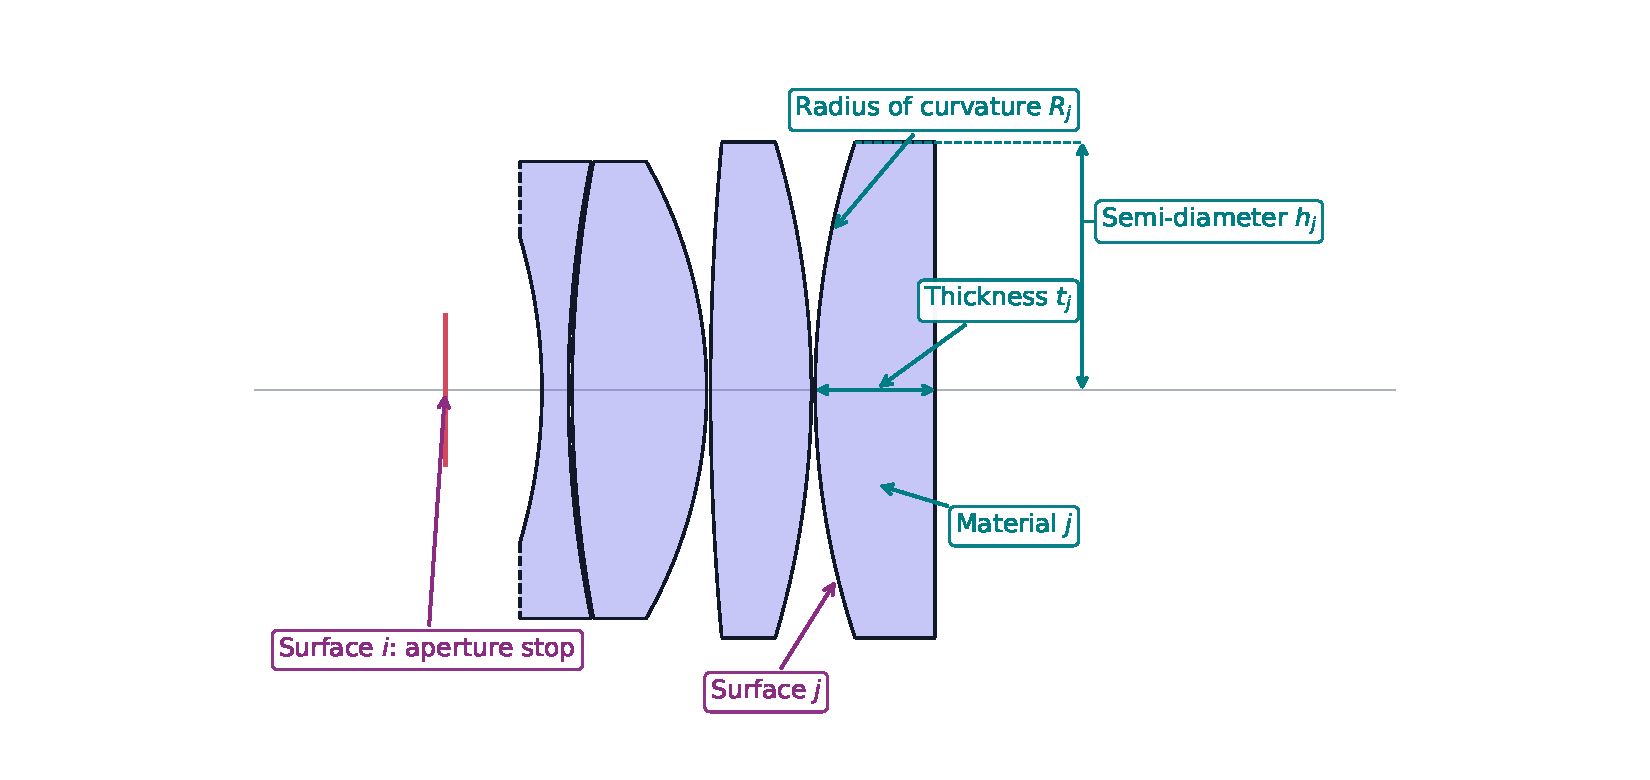
\includegraphics[width=0.85\linewidth]{figures/lens_params_def_programmatic/figure_2_patent_lens_parameters.pdf}
    \caption{\small\textbf{Lens system diagram with highlighted parameters.} A representative held-out patent-derived assembly is rendered from its prescription, with symbolic annotations for the surface radius of curvature, thickness, material, semi-diameter, surface index, and aperture-stop index used in the dataset representation.}
    \label{fig:lens_param}
\end{figure}

Along with design parameters, each optical system is associated with operating conditions that define its intended use:
\begin{enumerate}
    \item \textbf{Maximum field angle}: largest field angle to be accommodated by the system;
    \item \textbf{Effective focal length (EFL)}: target effective focal length;
    \item \textbf{Entrance pupil diameter (EPD)}: intended entrance pupil diameter;
    \item \textbf{Total length}: axial distance from the first surface to the image plane.
\end{enumerate}

The dataset also retains optical-performance annotations. The annotations used in this study include:
\begin{enumerate}
    \item \textbf{Spot-size metrics}: field-dependent spot-size measures such as SPO67 and SPO100;
    \item \textbf{Encircled-energy metrics}: field-dependent energy-concentration measures such as EE50 and EE90;
    \item \textbf{Axial nominal performance}: on-axis root-mean-square (RMS) wavefront error.
\end{enumerate}
Additional performance and sensitivity annotations are retained in the canonical dataset.\\
{\color{red}A complete inventory of the retained performance and sensitivity annotations will be added after the metric audit is completed.}
Unless otherwise specified, distances are reported in millimeters, angles in degrees, and wavelengths in nanometers.

\subsection{Patent Dataset Shortlisting}
\label{sec:dataset_patent_shortlisting}

To formulate a standardized starting point for generative modeling and synthetic dataset generation, we select and process designs from the collected reference corpus according to the following standardization and filtering criteria:
\begin{enumerate}
    \item Designs are specified for object distance of infinity.
    \item Materials are selected from existing optical material catalogues.
    \item Object and image spaces are air.
    \item Object and image surfaces are represented as flat/planar surfaces without curvature.
    \item Aspheric surfaces and gratings are not considered.
    \item The number of surfaces ranges from 3 to 17.
    \item A maximum field angle is used as a design specification.
    \item Design performance is evaluated at $\{0, 0.3, 0.5, 0.7, 1.0\}$ times the maximum field angle.
    \item Field angles are represented in the meridional/y-field direction, with x-field angle entries set to zero.
    \item Performance is evaluated in the visible spectrum using fixed wavelengths (F, d, C lines).
    \item The material between the last surface and image plane is air, and the penultimate material is glass.
\end{enumerate}

Applying these criteria gives a canonical subset of 1,253 confirmed patent designs selected from the broader 2,572-design patent-derived reference corpus. The retained rows keep the same tabular optical-prescription schema as the curated source corpus: non-applicable or structurally irrelevant cells are left empty, while fields affected by the standardization criteria are updated to the canonical form used for synthetic generation and modeling.\\
{\color{red}Detailed shortlisting counts from the collected patent corpus to the canonical patent subset need to be added after the source audit is finalized.}

\subsection{Synthetic Expansion}
\label{sec:dataset_synthetic_expansion}

The synthetic dataset is generated from the canonical patent subset using perturbations that preserve the tabular prescription format described above. This expansion is intended to increase the number and coverage of available optical prescriptions while keeping each synthetic row traceable to a realistic patent-derived design family. At a high level, the synthetic construction process is:
\begin{enumerate}
    \item sample a parent design from the canonical patent subset;
    \item perturb curvature, thickness, material, or combinations of these quantities;
    \item re-evaluate semi-diameters and image-plane placement using the optical evaluation pipeline;
    \item discard rows that fail the generation or simulation checks;
    \item retain successful rows with full lineage back to the parent design and perturbation source.
\end{enumerate}
Figure~\ref{fig:synth_data_pipe} summarizes this synthetic dataset construction workflow.

\begin{figure}[ht]
    \centering
    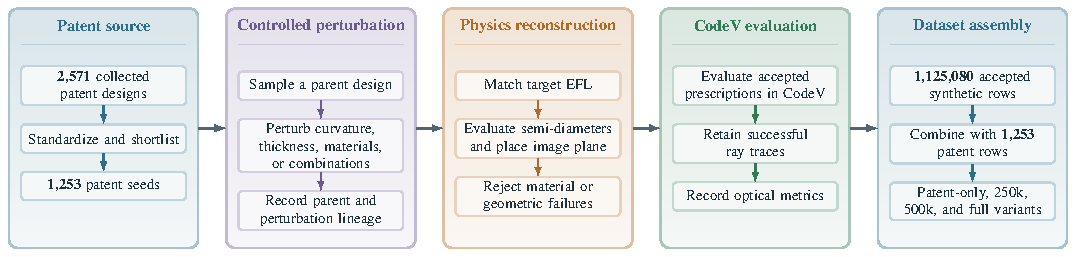
\includegraphics[width=\linewidth]{figures/synthetic_dataset_pipeline_tikz.pdf}
    \caption{\small\textbf{Synthetic dataset construction pipeline.} Patent-derived designs are standardized and shortlisted, perturbed with parent and perturbation lineage retained, reconstructed and filtered using optical checks, evaluated in CodeV, and assembled into the Patent-only, 250k, 500k, and full study datasets. Colors denote data artifacts (teal), controlled perturbation (purple), physics reconstruction (orange), and CodeV evaluation (green); arrows indicate forward data flow.}
    \label{fig:synth_data_pipe}
\end{figure}

The resulting canonical dataset contains 1,126,333 rows: 1,253 patent-derived rows and 1,125,080 synthetic rows. The synthetic rows are retained in the same tabular prescription format as the patent-derived rows and are generated through curvature, thickness, material, and combined perturbation families. Provenance fields are retained so that synthetic rows can be traced back to their parent patent designs and perturbation sources.

Figure \ref{fig:patent_synth_comp} summarizes patent-derived and synthetic dataset characteristics. Additional surface-count, condition-range, remaining-field optical-performance, and perturbation-lineage figures are provided in Appendix~\ref{app:dataset_details}, including Figure~\ref{fig:appendix_remaining_field_performance}.

\begin{figure}[t]
    \centering
    \begin{subfigure}[t]{0.48\linewidth}
        \centering
        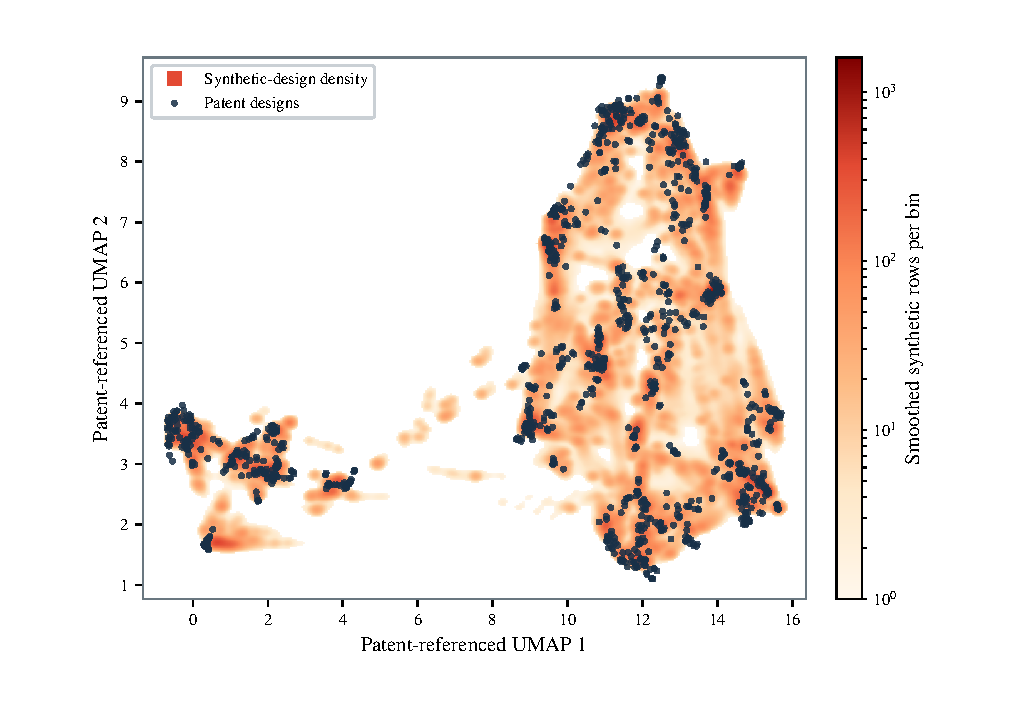
\includegraphics[width=\linewidth]{figures/mixed_landmark_umap_projection.pdf}
        \caption{Patent-referenced tuned-representation projection}
        \label{fig:patent_synth_comp_div}
    \end{subfigure}
    \hfill
    \begin{subfigure}[t]{0.48\linewidth}
        \centering
        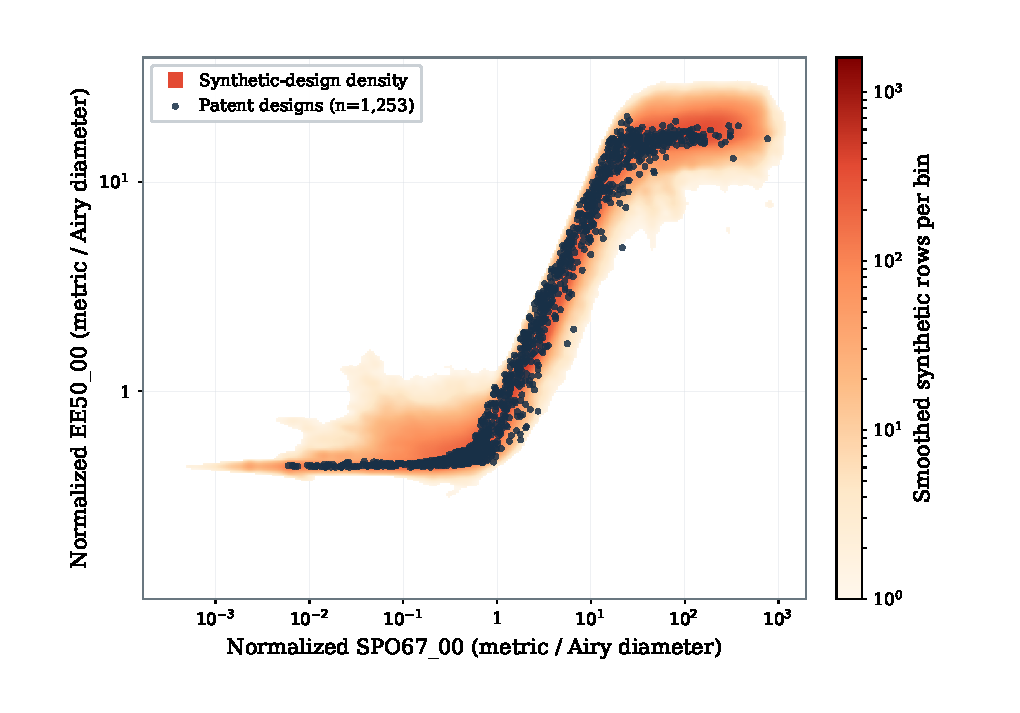
\includegraphics[width=\linewidth]{figures/normalized_ee50_vs_spo67.pdf}
        \caption{Normalized EE50 versus SPO67 comparison}
        \label{fig:patent_synth_comp_perf}
    \end{subfigure}
    \caption{\small\textbf{Patent-derived and synthetic dataset comparison.} Left: topology-aware projection used to compare coverage of patent-derived and synthetic designs. Right: normalized encircled-energy and spot-size comparison for optical-performance characterization.}
    \label{fig:patent_synth_comp}
\end{figure}


\section{Design Parameterization and Processing Pipeline}

Figure~\ref{fig:model_training_pipeline} summarizes the processing path used to move from canonical optical prescriptions to model-facing training tables and back to simulation-ready generated designs. The key design choice is to keep a single canonical prescription table as the dataset reference, then derive representation-specific tables for generative modeling. This separates optical data definition from model-specific formatting choices such as normalization, imputation, and file layout.

\begin{figure}[ht]
    \centering
    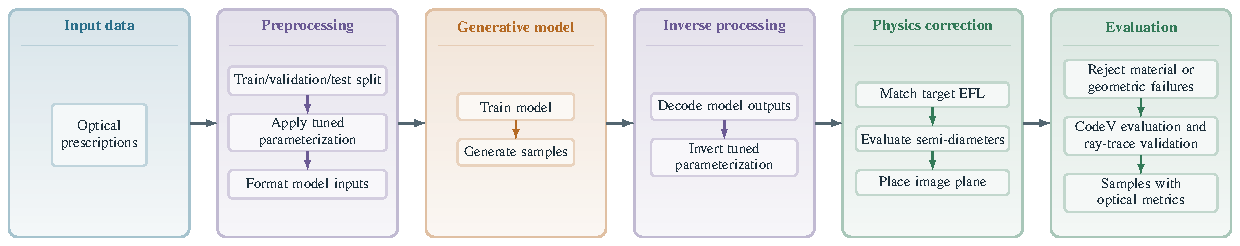
\includegraphics[width=\linewidth]{figures/model_processing_pipeline_filled_tikz.pdf}
    \caption{\textbf{Model-facing data and post-processing pipeline.} Optical prescriptions are partitioned, mapped into the tuned parameterization, formatted for model input, generated, and decoded. The inverse transform restores physical parameters before physics correction. Material or geometric failures are rejected before CodeV evaluation; successful ray traces provide optical metrics. Colors denote input data (teal), reversible deterministic transformations (purple), learned generation (orange), and optical correction and evaluation (green); arrows indicate forward data flow.}
    \label{fig:model_training_pipeline}
\end{figure}

\subsection{Canonical Table and Model-Facing Representations}
\label{sec:canonical_model_representations}

The canonical table stores each optical prescription in the common tabular schema introduced in the dataset section and detailed in Appendix~\ref{app:dataset_details}: surface geometry, material assignment, topology, design conditions, field and wavelength setup, optical-performance annotations, and provenance. Model-facing data are derived from this canonical table after separating prescription and design-condition variables from provenance columns, filtering flags, and optical-performance columns. The generative models are therefore trained on optical prescriptions and design conditions, not on the measured performance values that are reserved for evaluation.

We use two representation families. The \emph{untuned} representation keeps curvature, thickness, semi-diameter, and stop variables close to their canonical physical form and serves as the direct tabular baseline. The \emph{tuned} representation expresses curvature relative to system length, valid thicknesses as axial fractions with explicit system-length terms, semi-diameter relative to entrance-pupil diameter, and stop location relative to surface count. Both representations use continuous material-property coordinates with an explicit air indicator, preserve the same row order and split labels, and apply the same structural missingness mask. Appendix Table~\ref{tab:tuned_untuned_representation} provides the complete variable-by-variable comparison and inverse-processing rules.

For both representations, the material labels used for CodeV export are reconstructed after generation from the generated material variables. If a surface is marked as air, the air indicator takes priority over generated $N_d$ and $V_d$ values. Otherwise, generated material properties are projected to the nearest available catalog material. This keeps material generation continuous during modeling while returning to discrete material labels for optical simulation.

\subsection{Variable Surface Count and Structural Missingness}

Lens prescriptions have variable surface count, but the tabular benchmark models require a fixed column set. We therefore reserve surface-indexed columns up to the maximum supported surface count and use structural missing values for inactive surface slots. These missing values are not ordinary data gaps: they indicate that the corresponding surface does not exist for that design. During preprocessing, missing values inside active surface slots are treated as data-quality errors, while missing values outside the active surface count are preserved as structural padding. During post-processing, generated samples are re-masked using their generated surface count so that inactive surface slots remain empty before export.

The common representation layer also preserves row identity and split information, and writes provenance and performance information into sidecar artifacts rather than mixing them into the model-facing feature matrix. This makes the model-facing inputs and split assignments auditable without asking the generative model to learn source-folder, lineage, or performance-metric fields.

\subsection{Model-Specific Formatting and Normalization}

The common representation layer stops before model-specific numerical formatting. This is important for fair benchmarking: TabSyn, STaSY, CoDi, and other baselines can use the normalization, imputation, and mixed-type encodings required by their own training code, while starting from the same untuned or tuned optical representation. For example, quantile normalization is not part of the common representation definition; it is applied only when required by a particular benchmark implementation. This separation prevents model-specific preprocessing from being mistaken for an optical representation change.

\subsection{Generated-Sample Inverse Processing}

Generated samples are mapped back to canonical-style prescription tables before simulation. The inverse processor applies the paired inverse of the representation transform, restores deterministic field and wavelength defaults used by the canonical schema, reconstructs material labels from generated material variables, and re-applies the structural surface mask implied by the generated surface count. For generated rows, provenance sidecars from the training data are not copied row-by-row; only deterministic schema defaults and values inferable from the generated prescription are restored. This distinction is necessary because a generated batch does not share the row identity of the original training table.

\subsection{Physics-Based Post-Processing}

After inverse processing, generated prescriptions in the finalized pipeline pass through a ray-tracing-based correction layer before CodeV evaluation. This layer makes local optical corrections to the generated prescription rather than defining the training representation. The controlled ablation in Section~\ref{sec:results_raytrace_postproc} evaluates the same generated rows without this layer to isolate its contribution. The correction attempts the following stages:

\begin{enumerate}
    \item \textbf{Material and geometry precheck}: verify that active surfaces have valid material and geometry information before ray tracing is attempted.
    \item \textbf{Final-surface curvature tuning}: adjust the final active surface curvature to better match the generated target effective focal length using first-order ray-tracing estimates.
    \item \textbf{Semi-diameter evaluation}: recompute active-surface semi-diameters from traced rays while checking for geometric inconsistencies.
    \item \textbf{Image-plane placement}: adjust the final image gap using the traced focal location.
\end{enumerate}

The correction is applied stage by stage: a successful earlier correction can be retained even if a later correction is not available for a particular sample. Stage outcomes are recorded so that evaluation can compare generated prescriptions before and after ray-tracing correction using a common denominator.

\subsection{CodeV Preparation}

The final post-processed table is prepared as a CodeV-ready prescription table with canonical field, wavelength, material, surface, and image-plane columns. Sequence-file generation and CodeV execution are handled by the downstream simulation pipeline. This keeps the generative-model pipeline responsible for producing simulation-ready prescription tables, while the optical simulation pipeline remains responsible for generating sequence files, running CodeV, and returning optical-performance results.


\section{Benchmark Models And Evaluation Framework}
\label{sec:benchmark_models_evaluation}

This section defines the benchmark protocol used to evaluate whether optical prescription data can be modeled by modern generative methods and whether optics-aware processing improves generated design quality. We evaluate unconditional generation because it isolates distribution learning: the model must generate plausible lens prescriptions and design specifications without being given a target condition at sampling time.

\subsection{Benchmark Models}\label{subsec:off_shelf_uncond_gen}

The benchmark suite uses mixed-type tabular generative models as the primary unconditional baselines, including STaSY, CoDi, and TabSyn \cite{Kim2023STaSy,Lee2023CoDi,Zhang2024TabSyn}. These methods are appropriate baselines because the model-facing lens representations are stored as mixed numerical and categorical tables. At the same time, they do not natively encode optical surface ordering, variable surface count, aperture-stop structure, or ray-trace validity constraints. This makes them useful for testing how much benefit comes from the proposed data representation and post-processing pipeline.

For each model family, experiments are organized across the dataset variants in Table~\ref{tab:dataset_variants_splits} and across the untuned and tuned model-facing representations. In the benchmark artifacts used for the reported results, the canonical training and validation partitions are combined for model fitting, while the test partition remains held out. Model-specific processors are allowed to perform required formatting, imputation, and normalization, but these steps are recorded separately from the common representation layer. This separation is important because the common data representation is intended to define the optical variables, while model-specific processors define the input format required by a particular generative model implementation.

\begin{table}[t]
\centering
\small
\caption{\textbf{Dataset variants used for benchmark training and evaluation.} Training counts report the rows provided to benchmark-model training, and test counts report the held-out rows used for evaluation. Counts include both patent-derived and synthetic rows.}
\label{tab:dataset_variants_splits}
\begin{tabular}{lrrr}
\toprule
\textbf{Variant} & \textbf{Training rows} & \textbf{Held-out test rows} & \textbf{Total rows} \\
\midrule
Patent-only & 1,128 & 125 & 1,253 \\
Patent+Synth-250k & 362,114 & 112,642 & 474,756 \\
Patent+Synth-500k & 612,114 & 112,642 & 724,756 \\
Patent+Synth-full & 1,013,691 & 112,642 & 1,126,333 \\
\bottomrule
\end{tabular}
\end{table}

% \begin{table}[t]
% \centering
% \footnotesize
% \caption{\textcolor{red}{[placeholder table]} \textbf{Benchmark training protocol.} This table will be filled with the final model list, dataset variants, representation settings, and sampling counts used in the benchmark runs.}
% \label{tab:benchmark_protocol}
% \begin{tabular}{p{0.18\linewidth}p{0.20\linewidth}p{0.25\linewidth}p{0.25\linewidth}}
% \toprule
% \textbf{Model} & \textbf{Representation(s)} & \textbf{Dataset variant(s)} & \textbf{Role} \\
% \midrule
% TabSyn & Tuned, untuned & Patent-only, Patent+Synth-250k, Patent+Synth-500k, Patent+Synth-full & Main latent-diffusion tabular baseline \\
% STaSy & Tuned, untuned & Planned benchmark variants & Score-based tabular baseline \\
% CoDi & Tuned, untuned & Planned benchmark variants & Mixed-type contrastive diffusion baseline \\
% SMOTE-style interpolation & Tuned or untuned reference & Selected variants & Non-neural diversity/memorization reference \\
% \bottomrule
% \end{tabular}
% \end{table}

\subsection{Evaluation Stages}

Evaluation is separated into stages so that local generated-prescription quality is not conflated with CodeV/LLESP simulation outcomes. Before CodeV results are available, generated samples can be evaluated for table validity, material validity, geometric plausibility, distribution matching, diversity, novelty, and LLESP-readiness after deterministic post-processing. After CodeV/LLESP result files return, the same samples can be evaluated for simulation error rate and optical performance metrics.

For unconditional generation, design conditions such as EFL, EPD, and maximum field angle are treated as generated design specifications. Their distributions are compared against reference data, but they are not treated as target-satisfaction metrics because no requested target is supplied to the model at sampling time.

\subsection{Metric Families}

Distribution and diversity metrics are computed on prescription and design-condition columns, excluding optical performance columns such as spot size and encircled-energy metrics. Optical performance is evaluated only after ray tracing or CodeV/LLESP simulation has produced valid result files; detailed post-processing attrition counts can be reported in the appendix if needed.

% Internal planning table retained for reference but omitted from the rendered paper.
\begin{comment}
\begin{table}[t]
\centering
\footnotesize
\caption{\textbf{Evaluation metric groups.} Metrics are separated by evaluation stage so that generated-prescription validity, distributional fidelity, simulation robustness, optical performance, and ray-tracing post-processing benefit are evaluated without conflating distinct failure modes.}
\label{tab:evaluation_metric_groups}
\begin{tabular}{>{\raggedright\arraybackslash}p{0.18\linewidth}>{\raggedright\arraybackslash}p{0.33\linewidth}>{\raggedright\arraybackslash}p{0.15\linewidth}>{\raggedright\arraybackslash}p{0.22\linewidth}}
\toprule
\textbf{Metric family} & \textbf{Primary quantities} & \textbf{Stage} & \textbf{Claim supported} \\
\midrule
Prescription distribution & Surface-count distribution distance, active numerical marginal KS, active \texttt{isair} marginal error, and pairwise correlation error within surface-count groups & Pre-CodeV & Fidelity to reference design distributions \\
Novelty / train proximity & Same-surface-count DCR excess relative to the expected train-closer probability from train/test support sizes & Pre-CodeV & Train-proximity check after correcting for split-size imbalance \\
Duplicate and leakage checks & Exact or rounded duplicate rates, generated rows matching training rows, and parent-family split checks & Pre-CodeV & Defensible separation between training data and generated samples \\
Prescription validity & Active-surface masks, material no-match rate, geometric intersections, semi-diameter sanity, and LLESP-readiness & Post-processing / pre-CodeV & Fraction of generated prescriptions usable before simulation \\
CodeV/LLESP outcomes & Submitted rows, returned rows, \texttt{!error} rate, and simulation success/failure categories & CodeV-dependent & Simulation robustness of generated prescriptions \\
Optical performance & SPO67, SPO100, EE50, EE90, and axial nominal performance across evaluated fields & CodeV-dependent & Optical quality after simulation \\
Ray-tracing correction benefit & Paired feasible-fraction and optical-performance changes with and without physics-based post-processing & CodeV-dependent paired ablation & Effect of physics-based post-processing \\
\bottomrule
\end{tabular}
\end{table}
\end{comment}

For novelty and train-proximity diagnostics, nearest-neighbor comparisons are restricted to the same surface-count group. This avoids treating padded inactive surface slots as ordinary features and is equivalent to assigning cross-surface-count pairs a larger topology-aware distance than any same-surface-count pair. The reported DCR excess subtracts the expected train-closer probability implied by the same-surface-count train/test support sizes, so it is not interpreted against a fixed 50\% baseline unless the train and test supports are equal.


\section{Proposed conditional generative model}

We introduce a generative model framework with transformer-based auto-encoder and conditional latent diffusion model for the problem at hand. We further need to tokenize the parameter data that we have for the transformer model. Each of these components are explained in further detail in the below subsections.   

\subsection{Composite tokenizer}

For compatibility with transformer-based architectures, optical design parameters must be converted into sequence of tokens. Lens assembly can be characterized by a sequence of surfaces but each surface has a set of parameters as described in sub-section\ref{subsec:param_meth}. So each parameter is mapped to an individual token using the following process:
\begin{enumerate}
  \item \textbf{Initial embedding}
  \begin{enumerate}
    \item Numerical parameters are embedded using learnable affine projections
    \item Categorical parameters are embedded using lookup table 
  \end{enumerate}
  \item \textbf{Encoding parameter type} To enable the model to track parameter type of each token, a learnable parameter-type embedding (unique for each parameter type, same across surfaces) is added to each token based on associated parameter category.
  \item \textbf{Encoding surface position} 
  Surface ordering along the optical axis is also encoded using a relative fourier-based embedding. For the $i^{th}$ surface in a sytem with $N$ surfaces, a normalized position $\frac{i}{N-1}$ is computed and mapped to a set of sinusoidal fourier features, followed by a learned linear projection. The resulting embedding is added to the associated parameter tokens based on the surface number they belong to. 
  \item Aperture stop surface index is not included in the token sequence and instead  predicted at the decoder output using a dedicated regression head
\end{enumerate}

\subsection{Transformer based auto-encoder}
The overall encoder-decoder architecture follows a modified version of the standard transformer formulation introduced in \cite{vaswani2023attentionneed}, as shown in the figure \ref{fig:vasvani_trans}. The encoder operates on the tokens generated by the composite tokenizer described in the previous section, capturing both intra-surface parameter interactions and inter-surface relationships along optical axis. Rather than passing encoder outputs to the decoder, we aggregate them into a compact fixed dimensional latent representation using learned attention pooling. 

The decoder is implemented as an autoregressive transformer that takes in latent representation through cross-attention layers and reconstructs individual parameters in a surface-major, parameter-minor order. Furthermore, to prevent information leak, we use different instances of the described composite tokenizer for encoder and decoder. And,unlike the remaining surface parameters, stop surface index is predicted from the latent vector using a dedicated regression head. 

This auto-encoder architecture is then trained on the lens assembly design dataset with teacher forcing on the decoder side. The trained encoder is then used to sample the fixed length latent space mapping of all the training dataset designs 

\begin{figure}[ht]
    \centering
    % Set a clean publication-friendly size (not too large, not too small)
    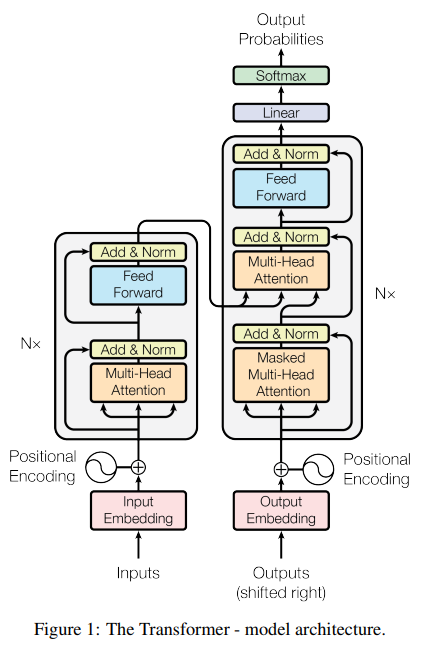
\includegraphics[width=0.5\linewidth]{figures/vasvani_transformer.png}

    % Improve caption formatting for papers
    \caption{A figure from \cite{vaswani2023attentionneed} showing the traditional encoder-decoder transformer architecture \textcolor{red}{[place holder - will add new architecture figure]}}
    \label{fig:vasvani_trans}
\end{figure}

\subsection{Conditional latent diffusion model}

Latent representations produced by the transformer-based auto-encoder are flattened and paired with their corresponding condition parameters to train a conditional diffusion model. We adopt the diffusion framework provided by the smalldiffusion package \cite{Yuan2025_smalldiffusion}, using its standard noise scheduling, training objectives, and sampling procedures. Modifications are introduced only in the conditioning mechanism and denoising network to enable modeling of multiple continuous design conditions.

In contrast to the standard neural network based denoising model implemented in the smalldiffusion package, we employ feature-wise linear modulation (FiLM) \cite{perez2017filmvisualreasoninggeneral}, to accommodate continuous design conditions. These condition values are first embedded using a small neural network and then passed on to FiLM layers for modulating the intermediate layer outputs.

This conditional diffusion model is then trained using the standard classifier-free guidance formulation implemented in the smalldiffusion package. Training minimizes a mean squared error loss between the predicted and true noise over a predefined noise schedule, with the conditioning inputs randomly dropped and replaced by a null condition. During inference, guided sampling is performed by combining conditional and unconditional predictions using a guidance scale, allowing explicit control over influence of conditioning. Generated latent samples are then reshaped to reverse flattening and are subsequently decoded using the decoder previously described, and put through the post-processing pipeline outlined in figure \ref{fig:model_training_pipeline}




\section{Results}

This section evaluates how generated tabular lens rows become usable optical prescriptions. Unless otherwise stated, each result starts from 10,000 generated samples. We report the \emph{simulation-verified feasible sample fraction}: the percentage of generated samples that pass post-processing and CodeV/LLESP preparation and then return from CodeV without an error. This denominator is stricter than a success rate on submitted samples because it also counts samples rejected before simulation. Log-whitened material-parameterization results and CoDi runs are excluded from the main results in this version.

\subsection{Synthetic-Expanded Training Data Improves Feasible Generation}
\label{sec:results_synthetic_expansion}

The first experiment asks whether the synthetic-expanded training set improves usable generation under the final pipeline. To isolate this effect, the representation is fixed to the tuned parameterization, NRTE post-processing is enabled, and each model is compared between patent-only training and the patent-plus-synthetic 250k training variant. Model hyperparameters are held fixed within each model family; the intended variable in this subsection is the training data source, not model size, representation, or post-processing.

\begin{center}
\begin{minipage}{0.98\linewidth}
\centering
\footnotesize
\captionof{table}{\textbf{Patent-only versus patent-plus-synthetic 250k feasible generation.} Deltas are absolute percentage-point changes from patent-only to 250k training. The dominant remaining failure mode is computed on the 250k run using mutually exclusive failure categories.}
\label{tab:section_6_1_synthetic_expansion_summary}
\begin{tabular}{lrrrl}
\toprule
\textbf{Model} & \multicolumn{2}{c}{\textbf{Feasible fraction $\uparrow$ (\%)}} & \textbf{$\Delta$ feasible} & \textbf{Dominant 250k failure} \\
\cmidrule(lr){2-3}
 & \textbf{Patent only} & \textbf{Patent+synth 250k} & \textbf{(pp)} & \\
\midrule
SMOTE-style reference & 81.40 & 98.43 & +17.03 & CodeV error \\
STaSy & 1.70 & 58.53 & +56.83 & Material only \\
TabDDPM & 0.00 & 0.00 & +0.00 & Material + geometry \\
TabSyn & 0.57 & 77.48 & +76.91 & Material only \\
\bottomrule
\end{tabular}
\end{minipage}
\end{center}

Table~\ref{tab:section_6_1_synthetic_expansion_summary} shows the feasible fraction for the four matched model families. The synthetic-expanded 250k dataset substantially increases the end-to-end feasible fraction for the learned tabular generators that can use the added data. TabSyn increases from 0.57\% feasible samples under patent-only training to 77.48\% under patent-plus-synthetic 250k training, and STaSy increases from 1.70\% to 58.53\%. The SMOTE-style reference is already highly feasible on patent-only training, but still increases from 81.40\% to 98.43\%. TabDDPM remains at 0.00\% feasible samples in both settings, showing that the benefit of synthetic-expanded training is not automatic across all tabular generators.

These results support two conclusions. First, the synthetic-expanded dataset is useful because the patent-only set is too small for several learned generators to produce simulation-ready prescriptions at meaningful rates. Second, feasibility must be measured after the optical reconstruction and simulation-readiness pipeline. A generator can produce rows that look tabularly valid while still failing material reconstruction, geometric consistency checks, or CodeV execution. The mutually exclusive failure-mode breakdown in Appendix~\ref{app:section_6_1_failure_breakdown} shows that the 250k runs reduce the large material-plus-geometry failure mass seen in the patent-only learned-model runs, but the remaining failure modes differ by generator: material-only failures dominate for STaSy and TabSyn, CodeV errors dominate the small residual failure rate for SMOTE, and TabDDPM remains dominated by coupled material and geometry failures.

\subsection{Effect Of Tuned Optical Representation}

The second experiment isolates the effect of the model-facing representation. The dataset is fixed to patent-plus-synthetic 250k, NRTE post-processing is enabled, and the comparison is restricted to model families with matched tuned and untuned returned runs. This keeps the intended variable as the optical representation rather than dataset size or post-processing.

Table~\ref{tab:tuned_untuned_results} shows that the tuned representation has little effect on the SMOTE-style reference but a large effect on TabSyn. For SMOTE, both representations submit nearly all generated rows to CodeV/LLESP and return nearly all submitted rows successfully, giving only a 0.36 percentage-point feasible-yield change. For TabSyn, the tuned and untuned branches submit nearly the same fraction of rows, 85.77\% versus 86.06\%, but their CodeV success rates among submitted rows differ sharply: 90.33\% for tuned versus 59.12\% for untuned. The resulting simulation-verified feasible fraction increases from 50.88\% to 77.48\%, a 26.60 percentage-point gain. This indicates that the tuned representation primarily improves the quality of reconstructed optical prescriptions that reach simulation, not merely the number of rows that pass the pre-CodeV gate.

\begin{center}
\begin{minipage}{0.98\linewidth}
\centering
\scriptsize
\setlength{\tabcolsep}{3pt}
\captionof{table}{\textbf{Tuned versus untuned representation comparison on patent-plus-synthetic 250k runs.} All entries use NRTE post-processing and the same 10,000-sample denominator. Deltas are tuned minus untuned in percentage points.}
\label{tab:tuned_untuned_results}
\begin{tabular}{lrrrrrrr}
\toprule
\textbf{Model} & \multicolumn{2}{c}{\textbf{CodeV input accepted (\%)}} & \multicolumn{2}{c}{\textbf{Success on submitted (\%)}} & \multicolumn{2}{c}{\textbf{Feasible fraction $\uparrow$ (\%)}} & \textbf{$\Delta$ feasible} \\
\cmidrule(lr){2-3}\cmidrule(lr){4-5}\cmidrule(lr){6-7}
 & \textbf{Tuned} & \textbf{Untuned} & \textbf{Tuned} & \textbf{Untuned} & \textbf{Tuned} & \textbf{Untuned} & \textbf{(pp)} \\
\midrule
SMOTE-style reference & 99.76 & 99.82 & 98.67 & 98.25 & 98.43 & 98.07 & +0.36 \\
TabSyn & 85.77 & 86.06 & 90.33 & 59.12 & 77.48 & 50.88 & +26.60 \\
\bottomrule
\end{tabular}
\end{minipage}
\end{center}

\subsection{Effect Of Synthetic Dataset Scale}

To isolate dataset scale from the representation ablation, Table~\ref{tab:dataset_scale_results} fixes the generator to TabSyn, the parameterization to the tuned representation, and the post-processing branch to NRTE. Since the paper-level question is how dataset scale changes the final usable sample population, the table reports the end-to-end feasible yield and a mutually exclusive breakdown of infeasible rows rather than intermediate pipeline gates.

The patent-only row is retained only as the low-data anchor. The main dataset effect is the transition from patent-only to patent-plus-synthetic training, where the feasible yield rises from 0.57\% to 77.48\%. Beyond 250k synthetic-expanded training rows, however, this fixed TabSyn configuration does not improve monotonically: the 500k run is comparable to 250k, while the full-dataset run falls to 67.15\%. The full-dataset run has higher material-only, material-plus-geometry, and CodeV-error fractions than the 250k run, so the drop is visible directly in the final infeasibility composition. Thus, the million-scale dataset is best interpreted as a released scaling endpoint and resource for higher-capacity or retuned models, not as a guarantee that the same off-the-shelf TabSyn configuration will be optimal at the largest scale.

\begin{center}
\begin{minipage}{0.98\linewidth}
\centering
\scriptsize
\setlength{\tabcolsep}{4.5pt}
\captionof{table}{Dataset-scale comparison for TabSyn with tuned representation and NRTE post-processing. Percentages are computed over 10{,}000 generated rows. Infeasibility categories are mutually exclusive and sum to the any-infeasible column.}
\label{tab:dataset_scale_results}
\begin{tabular}{lrrrrrr}
\toprule
\textbf{Training data} & \shortstack{\textbf{Feasible}\\\textbf{yield $\uparrow$}} & \shortstack{\textbf{Any}\\\textbf{infeasible $\downarrow$}} & \shortstack{\textbf{Material}\\\textbf{only $\downarrow$}} & \shortstack{\textbf{Geometry}\\\textbf{only $\downarrow$}} & \shortstack{\textbf{Material}\\\textbf{+ geom. $\downarrow$}} & \shortstack{\textbf{CodeV}\\\textbf{error $\downarrow$}} \\
\midrule
Patent only & 0.57 & 99.43 & 35.00 & 0.01 & 59.72 & 4.70 \\
Patent+synth 250k & 77.48 & 22.52 & 11.75 & 0.00 & 2.48 & 8.29 \\
Patent+synth 500k & 75.97 & 24.03 & 11.22 & 0.00 & 2.76 & 10.05 \\
Patent+synth full & 67.15 & 32.85 & 15.75 & 0.00 & 4.59 & 12.51 \\
\bottomrule
\end{tabular}
\end{minipage}
\end{center}

\subsection{Ray-Tracing Based Post-Processing Benefit}
\label{sec:results_raytrace_postproc}

The final ablation evaluates the optional ray-tracing based post-processing layer. The generator, representation, and training data are fixed to TabSyn with the tuned representation on the patent-plus-synthetic 250k training variant. The only intended variable is whether generated prescriptions pass directly to CodeV/LLESP preparation or first pass through NRTE.

NRTE increases the end-to-end feasible yield from 66.52\% to 77.48\%, a gain of 10.96 percentage points under the same 10{,}000-sample denominator (Table~\ref{tab:raytrace_postproc_benefit}). This shows that the deterministic correction layer adds simulation-verified usable designs without retraining the generator.

\begin{center}
\begin{minipage}{0.98\linewidth}
\centering
\footnotesize
\setlength{\tabcolsep}{6pt}
\captionof{table}{\textbf{Effect of ray-tracing based post-processing on TabSyn tuned 250k generated samples.} Delta is NRTE minus no-NRTE in percentage points, with the same 10{,}000-sample denominator used for both branches.}
\label{tab:raytrace_postproc_benefit}
\begin{tabular}{lrrr}
\toprule
\textbf{Dataset} & \multicolumn{2}{c}{\textbf{Feasible fraction $\uparrow$ (\%)}} & \textbf{$\Delta$ feasible $\uparrow$ (pp)} \\
\cmidrule(lr){2-3}
 & \textbf{No NRTE} & \textbf{NRTE} & \textbf{NRTE--no NRTE} \\
\midrule
Patent+synth 250k & 66.52 & 77.48 & +10.96 \\
\bottomrule
\end{tabular}
\end{minipage}
\end{center}

Feasibility alone does not show whether the correction damages optical quality. Figure~\ref{fig:results_nrte_metric_improvement_distribution_250k} therefore compares paired optical metrics on common rows that were submitted in both branches and returned successfully in both CodeV runs. The plotted value is $\log_{10}(\mathrm{no\ NRTE}/\mathrm{NRTE})$ for each field-metric observation; positive values indicate lower metric values after NRTE. Spot-size and encircled-energy metrics are normalized by the corresponding Airy diameter before comparison, while the nominal performance metric is left in its returned units. This paired comparison is a within-sample post-processing diagnostic rather than a ranking of unrelated generated designs.

\begin{center}
    \includegraphics[width=\linewidth]{../../../code/optics_data_modder_2/results/figures/paper_section_6_4_paired_metric_improvements_250k_20260522/section_6_4_paired_metric_improvement_violin_250k.pdf}
    \captionof{figure}{\textbf{Paired optical-metric improvement distributions after NRTE for TabSyn tuned 250k generations.} Each distribution pools the five evaluated field positions over common rows that succeeded in both CodeV/LLESP branches. Positive values indicate lower metric values after NRTE. SPO67, SPO100, EE50, and EE90 are normalized by the Airy diameter; nominal performance is not Airy-normalized.}
    \label{fig:results_nrte_metric_improvement_distribution_250k}
\end{center}

Table~\ref{tab:raytrace_postproc_quality_250k} reports the corresponding median values and paired improvement fractions. NRTE reduces the median normalized SPO67 from 168.24 to 22.95, normalized SPO100 from 285.18 to 57.59, and nominal performance from 11.76 to 2.73. The median reductions for EE50 and EE90 are smaller but remain positive, and 73.2--75.9\% of valid field-metric observations improve. Field-resolved median reductions are provided in Appendix~\ref{app:raytrace_metric_delta_details}.

\begin{center}
\begin{minipage}{0.98\linewidth}
\centering
\scriptsize
\setlength{\tabcolsep}{4pt}
\captionof{table}{\textbf{Paired optical-quality summary for TabSyn tuned 250k samples with and without NRTE.} $N$ is the number of valid paired field-metric observations after requiring common rows, successful CodeV/LLESP returns in both branches, and positive finite metric values. Percent reduction is $100 \times (\mathrm{no\ NRTE} - \mathrm{NRTE})/\mathrm{no\ NRTE}$ computed per paired observation and then summarized by the median.}
\label{tab:raytrace_postproc_quality_250k}
\begin{tabular}{lrrrrr}
\toprule
\textbf{Metric} & \textbf{$N$} & \textbf{Median no NRTE} & \textbf{Median NRTE} & \textbf{Median reduction $\uparrow$ (\%)} & \textbf{Improved rows $\uparrow$ (\%)} \\
\midrule
SPO67 / Airy diameter & 30{,}415 & 168.24 & 22.95 & 81.1 & 89.7 \\
SPO100 / Airy diameter & 30{,}415 & 285.18 & 57.59 & 71.8 & 85.5 \\
EE50 / Airy diameter & 30{,}412 & 15.64 & 11.50 & 31.0 & 75.9 \\
EE90 / Airy diameter & 30{,}408 & 22.37 & 20.08 & 23.8 & 73.2 \\
Nominal performance & 31{,}776 & 11.76 & 2.73 & 70.9 & 81.6 \\
\bottomrule
\end{tabular}
\end{minipage}
\end{center}


\input{sections/conclusions.tex}

\bibliographystyle{unsrtnat}
\bibliography{references}  %%% Uncomment this line and comment out the ``thebibliography'' section below to use the external .bib file (using bibtex) .


%%% Uncomment this section and comment out the \bibliography{references} line above to use inline references.
% \begin{thebibliography}{1}

% 	\bibitem{kour2014real}
% 	George Kour and Raid Saabne.
% 	\newblock Real-time segmentation of on-line handwritten arabic script.
% 	\newblock In {\em Frontiers in Handwriting Recognition (ICFHR), 2014 14th
% 			International Conference on}, pages 417--422. IEEE, 2014.

% 	\bibitem{kour2014fast}
% 	George Kour and Raid Saabne.
% 	\newblock Fast classification of handwritten on-line arabic characters.
% 	\newblock In {\em Soft Computing and Pattern Recognition (SoCPaR), 2014 6th
% 			International Conference of}, pages 312--318. IEEE, 2014.

% 	\bibitem{keshet2016prediction}
% 	Keshet, Renato, Alina Maor, and George Kour.
% 	\newblock Prediction-Based, Prioritized Market-Share Insight Extraction.
% 	\newblock In {\em Advanced Data Mining and Applications (ADMA), 2016 12th International 
%                       Conference of}, pages 81--94,2016.

% \end{thebibliography}

\appendix

\section{Dataset Details}
\label{app:dataset_details}

This appendix documents the schema, selection rules, construction counts, lineage, and descriptive statistics supporting Section~\ref{sec:dataset_patent_reference}--\ref{sec:dataset_synthetic_expansion}. Counts are taken from the finalized patent snapshot, the consolidated synthetic-data processing summary, and the canonical dataset manifests used in the reported experiments.

\subsection{Canonical Schema and CodeV Annotations}
\label{app:dataset_schema}

The canonical table preserves the optical prescription, simulation specification, evaluated descriptors, and provenance in separate column groups. In Table~\ref{tab:canonical_column_groups}, \texttt{XY} denotes a zero-based surface index and \texttt{0X} denotes a field or wavelength index. Empty surface-indexed cells outside the active surface count represent structural absence rather than missing measurements.

\small
\begin{longtable}{@{}p{0.22\textwidth}p{0.25\textwidth}p{0.46\textwidth}@{}}
\caption{Principal column groups in the canonical optical-prescription table.}\label{tab:canonical_column_groups}\\
\toprule
\textbf{Columns or pattern} & \textbf{Quantity} & \textbf{Units and role} \\
\midrule
\endfirsthead
\multicolumn{3}{l}{\textit{Table~\thetable\ continued}}\\
\toprule
\textbf{Columns or pattern} & \textbf{Quantity} & \textbf{Units and role} \\
\midrule
\endhead
\midrule
\multicolumn{3}{r}{\textit{Continued on next page}}\\
\endfoot
\bottomrule
\endlastfoot
\texttt{sXY\_00} & Signed surface radius of curvature & Prescription length unit recorded by \texttt{dim}; primary surface-geometry variable. \\
\texttt{sXY\_01} & Axial distance to the next surface & Prescription length unit recorded by \texttt{dim}; primary surface-geometry variable. \\
\texttt{sXY\_02} & Material following the surface & Catalog label or air; primary surface-material variable. \\
\texttt{sXY\_cir\_00} & Circular aperture semi-diameter & Prescription length unit recorded by \texttt{dim}; evaluated or supplied surface aperture. \\
\texttt{sXY\_k\_00}, \texttt{sXY\_[a--j]\_00} & Conic constant and even-order $A_4$--$A_{20}$ coefficients & Retained for aspheric source designs; absent from the all-spherical canonical subset. \\
\texttt{xan00\_0X}, \texttt{yan00\_0X} & Chief-ray field angle & degrees; one supported field-specification convention. \\
\texttt{xri00\_0X}, \texttt{yri00\_0X}; \texttt{xim00\_0X}, \texttt{yim00\_0X}; \texttt{xob00\_0X}, \texttt{yob00\_0X} & Real-image, paraxial-image, or object-height field specification & mm; alternative source-dependent field conventions. Only the convention used by a design is populated. \\
\texttt{fldx\_0X}, \texttt{fldy\_0X} & Evaluated half field of view & degrees at the reference wavelength. \\
\texttt{wl00\_0X}, \texttt{wtw00\_0X}, \texttt{ref00\_00} & Wavelength, relative weight, and reference-wavelength index & nm, unitless weight, and one-based index, respectively. \\
\texttt{so00\_*}, \texttt{si00\_*} & Object- and image-surface prescription & Radius and axial distance use the prescription length unit recorded by \texttt{dim}; material fields follow the physical-surface convention. \\
\texttt{epd}, \texttt{fno}, \texttt{sto}, \texttt{dim} & Aperture and global setup & Entrance-pupil diameter in the recorded prescription length unit, f-number, stop-surface index, and prescription length unit. \\
\texttt{efl}, \texttt{bfl}, \texttt{oal}, \texttt{lens2img}, \texttt{totlenstrack}, \texttt{objdist}, \texttt{minlenssep}, \texttt{diy} & First-order, packaging, object-distance, separation, and distortion descriptors & Distance-valued fields use the prescription length unit recorded by \texttt{dim}; evaluated by CodeV or derived analytically as appropriate. \\
\texttt{elemcount}, \texttt{cemlenscount}, \texttt{asphcount}, \texttt{surfcount}, \texttt{isintstop} & Structural descriptors & Counts and an internal-stop indicator. \\
\texttt{spo67\_0X}, \texttt{spo100\_0X} & Centroid-referenced polychromatic RMS and full geometric spot diameters & Prescription length unit recorded by \texttt{dim}; diffraction excluded. \\
\texttt{ee50\_0X}, \texttt{ee90\_0X} & Centroid-referenced polychromatic encircled-energy measures & Diffraction-aware CodeV outputs; normalized by Airy diameter for the comparisons in this paper. \\
\texttt{nomperf\_0X} & RMS wavefront aberration & waves at the reference wavelength. \\
\texttt{perfsens\_0X}, \texttt{tolsens\_0X}, \texttt{normalignsens} & Performance, relative tolerance, and alignment sensitivity annotations & CodeV evaluation outputs retained for analysis; they are not generative-model inputs or primary outcome metrics in this study. \\
\texttt{Seq File}, \texttt{dataset\_row\_id}, source-, parent-, perturbation-, and split-related columns & Artifact identity and provenance & Connects each table row to its sequence file, source record, patent family, perturbation record, and benchmark partition. \\
\end{longtable}
\normalsize

In the full patent-derived corpus, the prescription length unit is recorded for each row by \texttt{dim}. The shortlisted patent and synthetic tables are standardized to millimeters. Unless otherwise stated, angles are reported in degrees and wavelengths in nanometers. Optical-performance annotations are excluded from the model-facing feature matrices and used only for filtering, characterization, or post-simulation evaluation.

\subsection{Synthetic Lineage and Traceability}
\label{app:synthetic_lineage_details}

Table~\ref{tab:perturbation_method_counts} reports the final synthetic rows by perturbation family.

\begin{table}[htbp]
\centering
\small
\caption{Perturbation lineage in the final synthetic dataset.}
\label{tab:perturbation_method_counts}
\begin{tabular}{lrr}
\toprule
\textbf{Perturbation method} & \textbf{Rows} & \textbf{Fraction} \\
\midrule
Thickness & 226,846 & 20.2\% \\
Curvature & 185,299 & 16.5\% \\
Thickness + curvature & 179,298 & 15.9\% \\
Material & 140,534 & 12.5\% \\
Thickness + material & 133,733 & 11.9\% \\
Curvature + material & 129,943 & 11.5\% \\
Thickness + curvature + material & 129,427 & 11.5\% \\
\bottomrule
\end{tabular}
\end{table}

The canonical tables retain the lineage groups in Table~\ref{tab:traceability_fields}. These fields remain outside the default model-facing matrices and support source auditing, family-safe splitting, and post-hoc stratification.

\begin{table}[htbp]
\centering
\small
\caption{Traceability fields retained with canonical rows.}
\label{tab:traceability_fields}
\begin{tabular}{@{}p{0.25\linewidth}p{0.67\linewidth}@{}}
\toprule
\textbf{Field group} & \textbf{Representative columns} \\
\midrule
Dataset identity & \texttt{dataset\_row\_id}, \texttt{source\_type}, and \texttt{split}. \\
Source record & \texttt{source\_folder}, \texttt{source\_row\_id}, \texttt{source\_regen\_csv}, and \texttt{source\_submitted\_csv}. \\
Sequence file & \texttt{Seq File}, \texttt{source\_seq\_file\_index}, and \texttt{source\_seq\_file\_basename}. \\
Patent parent & \texttt{parent\_patent\_id}, \texttt{parent\_patent\_row\_id}, and \texttt{parent\_patent\_seq\_file\_basename}. \\
Perturbation & \texttt{perturb\_seed}, \texttt{perturb\_method}, and the curvature-, thickness-, and material-use indicators. \\
Canonical filtering & \texttt{passes\_common\_filters}, \texttt{rejection\_reasons}, and \texttt{filter\_drop\_*}. \\
\bottomrule
\end{tabular}
\end{table}

\subsection{Dataset Characteristics}
\label{app:dataset_characteristics}

Table~\ref{tab:appendix_dataset_characteristics} summarizes the principal ranges. Figures~\ref{fig:appendix_surface_count_distribution} and~\ref{fig:appendix_condition_distributions} compare topology and operating conditions, and Figure~\ref{fig:appendix_remaining_field_performance} extends the axial performance comparison in Figure~\ref{fig:patent_synth_comp} to the remaining field positions.

\begin{table}[htbp]
\centering
\small
\caption{Patent-derived and synthetic dataset characteristics. Percentile entries report the 5th--95th percentile interval.}
\label{tab:appendix_dataset_characteristics}
\begin{tabular}{lrr}
\toprule
\textbf{Characteristic} & \textbf{Patent-derived} & \textbf{Synthetic} \\
\midrule
Rows & 1,253 & 1,125,080 \\
Represented parent families & 1,253 & 1,251 \\
Surface-count range; median & 3--17; 11 & 3--17; 11 \\
EFL (mm) & 1.0--199.9 & 1.0--179.9 \\
EPD (mm) & 0.2--71.4 & 0.2--60.7 \\
Maximum field angle (deg) & 2.7--40.0 & 2.9--38.0 \\
Image gap (mm) & 1.0--316.4 & 1.0--325.9 \\
Minimum lens separation (mm) & 0.002--3.501 & 0.002--3.500 \\
\bottomrule
\end{tabular}
\end{table}

\begin{figure}[htbp]
\centering
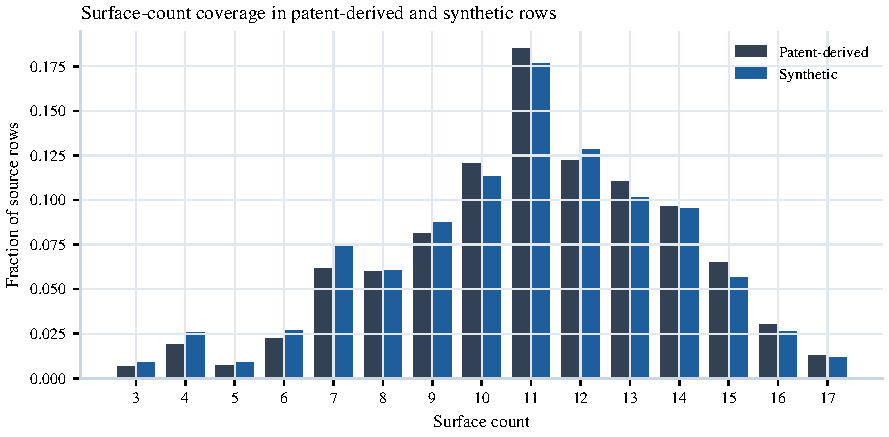
\includegraphics[width=0.88\linewidth]{figures/dataset_surface_count_distribution.pdf}
\caption{\textbf{Surface-count distribution.} Patent-derived and synthetic designs both span 3--17 active surfaces, with a median of 11. Bars show the fraction within each source type rather than raw counts.}
\label{fig:appendix_surface_count_distribution}
\end{figure}

\begin{figure}[htbp]
\centering
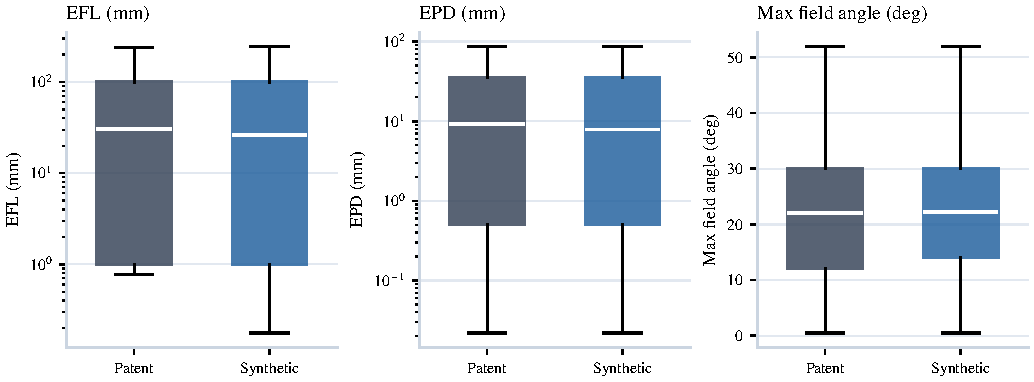
\includegraphics[width=0.9\linewidth]{figures/dataset_design_condition_distributions.pdf}
\caption{\textbf{Design-condition distributions.} Effective focal length, entrance-pupil diameter, and maximum field angle are compared between patent-derived and synthetic designs. The EFL and EPD axes are logarithmic.}
\label{fig:appendix_condition_distributions}
\end{figure}

\begin{figure}[htbp]
\centering
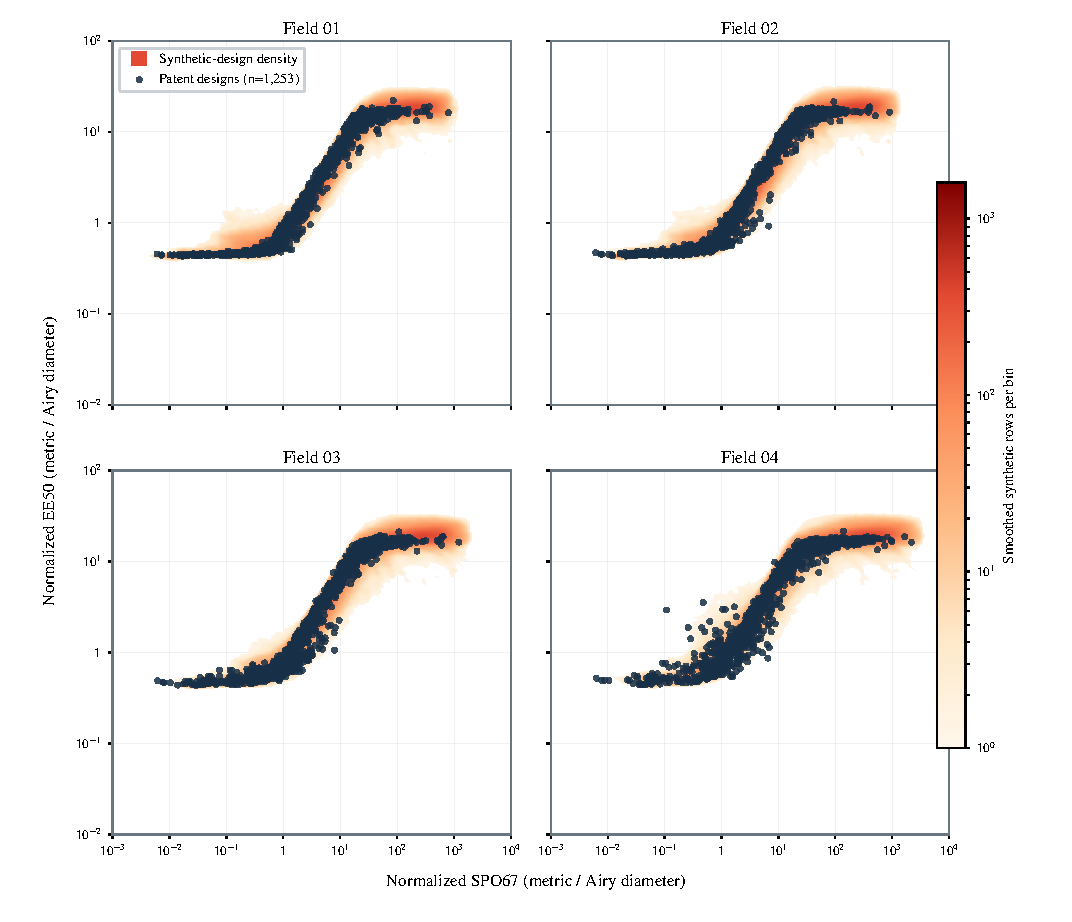
\includegraphics[width=0.95\linewidth]{figures/normalized_ee50_vs_spo67_remaining_fields_appendix.pdf}
\caption{\textbf{Off-axis optical-performance distributions.} Airy-normalized EE50 and SPO67 are shown at the four non-axial field positions. Patent designs are overlaid on the smoothed synthetic-design density, and both axes use logarithmic scaling.}
\label{fig:appendix_remaining_field_performance}
\end{figure}

\section{Model-Facing Dataset Details}

\subsection{Untuned and Tuned Representations}

Table~\ref{tab:tuned_untuned_representation} expands the distinction between the two model-facing representations summarized in Section~\ref{sec:canonical_model_representations}.

\begin{table}[htbp]
\centering
\small
\caption{Untuned and tuned model-facing representations. Both are derived from the same canonical rows and preserve row order and split labels.}
\label{tab:tuned_untuned_representation}
\begin{tabular}{@{}p{0.19\linewidth}p{0.35\linewidth}p{0.38\linewidth}@{}}
\toprule
\textbf{Quantity} & \textbf{Untuned representation} & \textbf{Tuned representation} \\
\midrule
Material & Catalog labels mapped to continuous $N_d$ and $V_d$ coordinates with air indicated explicitly. & The same continuous $N_d$ and $V_d$ coordinates and explicit air indicator. \\
Surface shape & Signed radius of curvature in physical units. & Signed curvature scaled by total system length. \\
Axial spacing & Inter-surface thickness in millimeters. & Valid inter-surface distances as axial fractions, with explicit system-length and image-gap terms. \\
Semi-diameter & Physical semi-diameter in millimeters. & Semi-diameter normalized by entrance-pupil diameter. \\
Aperture stop & Raw stop-surface index treated as categorical topology. & Stop position normalized by surface count and treated as a numerical topology variable. \\
Inactive surfaces & Structural missing values outside the active surface count. & The same structural missingness mask. \\
Inverse processing & Restores export defaults and the structural mask. & Inverts material, curvature, thickness, semi-diameter, and stop transforms before export and restores the structural mask. \\
\bottomrule
\end{tabular}
\end{table}

\subsection{Benchmark Split Source Counts}

Patent families are assigned to partitions before dataset-size variants are formed, keeping each patent and its synthetic descendants in one partition. The benchmark artifacts used for the reported models combine the canonical training and validation partitions into the model-training table; the test partition remains held out. Table~\ref{tab:canonical_split_source_breakdown} gives the resulting source counts. Synthetic validation and test rows are fixed across the 250k, 500k, and full variants; the size label counts sampled synthetic training rows only.

\begin{table}[htbp]
\centering
\footnotesize
\setlength{\tabcolsep}{4pt}
\caption{Patent-derived and synthetic rows in the benchmark training and held-out test tables.}
\label{tab:canonical_split_source_breakdown}
\begin{tabular}{lrrrrrr}
\toprule
\textbf{Variant} & \multicolumn{3}{c}{\textbf{Training rows}} & \multicolumn{3}{c}{\textbf{Held-out test rows}} \\
\cmidrule(lr){2-4}\cmidrule(lr){5-7}
 & \textbf{Patent} & \textbf{Synthetic} & \textbf{Total} & \textbf{Patent} & \textbf{Synthetic} & \textbf{Total} \\
\midrule
Patent-only & 1,128 & 0 & 1,128 & 125 & 0 & 125 \\
Patent+Synth-250k & 1,128 & 360,986 & 362,114 & 125 & 112,517 & 112,642 \\
Patent+Synth-500k & 1,128 & 610,986 & 612,114 & 125 & 112,517 & 112,642 \\
Patent+Synth-full & 1,128 & 1,012,563 & 1,013,691 & 125 & 112,517 & 112,642 \\
\bottomrule
\end{tabular}
\end{table}

\section{Benchmark Result Details}
\label{app:benchmark_result_details}

\subsection{Synthetic-Expansion Outcome Breakdown}
\label{app:section_6_1_failure_breakdown}

The main Section~\ref{sec:results_synthetic_expansion} reports feasible sample fractions for Patent-only and Patent+Synth-full training under the tuned representation with physics-based post-processing. Table~\ref{tab:appendix_section_6_1_failure_breakdown} provides the corresponding preparation and CodeV outcome breakdown. The outcome categories are computed over the same 10{,}000 generated rows per model/dataset/seed run and then averaged across four sampling seeds. Pre-CodeV rejected rows fail before submission to CodeV/LLESP, CodeV error rows are submitted but return with an error, and feasible rows are submitted and return successfully.

\begin{table}[htbp]
\centering
\scriptsize
\setlength{\tabcolsep}{4pt}
\caption{\textbf{Outcome composition for Section~\ref{sec:results_synthetic_expansion}.} Values are mean percentages of generated rows across four sampling seeds and sum to approximately 100\% for each row.}
\label{tab:appendix_section_6_1_failure_breakdown}
\begin{tabular}{llrrr}
\toprule
\textbf{Model} & \textbf{Training data} & \shortstack{\textbf{Pre-CodeV}\\\textbf{rejected}} & \shortstack{\textbf{CodeV}\\\textbf{error}} & \shortstack{\textbf{Feasible}\\\textbf{rows}} \\
\midrule
CoDi & Patent-only & 10.82 & 82.09 & 7.09 \\
CoDi & Patent+Synth-full & 4.69 & 38.74 & 56.57 \\
SMOTE-style reference & Patent-only & 0.00 & 13.16 & 86.84 \\
SMOTE-style reference & Patent+Synth-full & 0.18 & 1.52 & 98.30 \\
STaSY & Patent-only & 31.27 & 68.20 & 0.54 \\
STaSY & Patent+Synth-full & 6.84 & 16.66 & 76.50 \\
TabSyn ($3\times10^{-4}$) & Patent-only & 7.07 & 74.31 & 18.62 \\
TabSyn ($3\times10^{-4}$) & Patent+Synth-full & 1.55 & 14.73 & 83.72 \\
\bottomrule
\end{tabular}
\end{table}

\subsection{Ray-Tracing Post-Processing Metric Details}
\label{app:raytrace_metric_delta_details}

Section~\ref{sec:results_raytrace_postproc} reports the controlled ablation with and without physics-based post-processing using the seed-averaged paired heatmap and aggregate summary table. All distributions use the Patent+Synth-full TabSyn tuned run with diffusion learning rate $3\times10^{-4}$. Across the four sampling seeds, the branch without post-processing has 6{,}730 \ensuremath{\pm} 47 feasible rows and the branch with post-processing has 8{,}372 \ensuremath{\pm} 28 feasible rows out of the same 10{,}000 generated-row denominator. SPO and encircled-energy metrics are normalized by Airy diameter; nominal performance is left in its returned units.


\end{document}
